\documentclass[aspectratio=169,11pt]{beamer}

% ================================================================
% "TABIIY TILNI QAYTA ISHLASH" KURSI — MA'RUZA SHABLONI (v1.0)
% ================================================================
% Bu fayl — kursning BARCHA ma'ruzalari uchun namunaviy shablon.
% Vizual identifikatsiya (ranglar, shakllar, footer) asl fayldan
% O'ZGARISHSIZ olingan. Yangilik — pedagogik SKELET:
%
%   [A] Titul
%   [B] O'tgan darsdan ko'prik (retrieval practice — 2 savol)
%   [C] Bugungi maqsadlar (o'lchanadigan natijalar) + talablar
%   [D] Reja + vaqt taqsimoti
%   [E] Motivatsiya: avval MUAMMO, keyin usul
%   --- har bir bo'lim (section) uchun takrorlanuvchi naqsh: ---
%   [F] Intuitsiya (avval rasm, keyin formula)
%   [G] Formal ta'rif + belgilashlar kaliti ("bunda: ...")
%   [H] Keltirib chiqarish (derivation) — qadam-baqadam
%   [I] Qo'lda hisoblangan misol
%   [J] "Sizning vazifangiz" (savol -> pauza -> javob)
%   [K] Kod <-> formula ko'prigi (raqamlangan moslik)
%   [L] Cheklovlar va tipik xatolar
%   [M] O'zbek tiliga xoslik
%   ----------------------------------------------------------------
%   [N] Sintez: usullarni taqqoslash jadvali
%   [O] Ilmiy manba: asl maqola + muhokama savoli
%   [P] Xulosa: maqsadlarga qaytish
%   [Q] Ertangi amaliyotga ko'prik
%   [R] Adabiyotlar
%   [S] Zaxira slaydlar (\appendix dan keyin)
%
% QOIDALAR (har bir ma'ruza uchun):
%   1) Bir slayd — bir g'oya. Slayd sarlavhasi gap bo'lsin
%      ("TF-IDF" emas, "TF-IDF kam uchraydigan so'zni mukofotlaydi").
%   2) Har bir formula uchun "bunda:" kaliti majburiy.
%   3) Har bir nazariy blokdan keyin <= 3 slayd ichida misol/vazifa.
%   4) Har kod slaydi formuladagi qaysi qatorga mosligini ko'rsatsin.
%   5) 80 daqiqa ~ 22--28 slayd (zaxiradan tashqari).
% ================================================================

% ================================================================
% RANGLAR  (asl fayldan o'zgarishsiz)
% ================================================================
\definecolor{cnublue}{rgb}{0.07,0.14,0.62}
\definecolor{cnubluelight}{rgb}{0.18,0.30,0.72}
\definecolor{cnubluebg}{rgb}{0.90,0.92,0.97}
\definecolor{deepblue}{rgb}{0.07,0.14,0.62}
\definecolor{deepred}{rgb}{0.60,0.00,0.00}
\definecolor{deepgreen}{rgb}{0.00,0.45,0.00}
\definecolor{halfgray}{gray}{0.55}

% ================================================================
% BEAMER MAVZU — Boadilla + maxsus footer  (asl fayldan o'zgarishsiz)
% ================================================================
\usetheme{Boadilla}

\setbeamercolor{structure}{fg=cnublue}
\setbeamercolor{frametitle}{bg=cnublue,fg=white}
\setbeamercolor{title}{bg=cnublue,fg=white}
\setbeamercolor{block title}{bg=cnublue,fg=white}
\setbeamercolor{block body}{bg=cnubluebg,fg=black}
\setbeamercolor{alerted text}{fg=deepred}
\setbeamercolor{author in head/foot}{bg=cnubluelight,fg=white}
\setbeamercolor{section in head/foot}{bg=cnublue,fg=white}
\setbeamercolor{page number in head/foot}{bg=cnubluelight,fg=white}

\setbeamertemplate{mini frame}{}
\setbeamertemplate{mini frame in current section}{}
\setbeamertemplate{mini frame in current subsection}{}
\setbeamertemplate{headline}{}
\setbeamertemplate{navigation symbols}{}

\setbeamertemplate{footline}{%
  \leavevmode%
  \hbox{%
    \begin{beamercolorbox}[wd=0.17\paperwidth,ht=2.5ex,dp=1.25ex,leftskip=0.5em]{author in head/foot}%
      \usebeamerfont{author in head/foot}\scriptsize\insertshortauthor%
    \end{beamercolorbox}%
    \begin{beamercolorbox}[wd=0.69\paperwidth,ht=2.5ex,dp=1.25ex,center]{section in head/foot}%
      \usebeamerfont{section in head/foot}%
      \scriptsize\insertsectionnavigationhorizontal{0.69\paperwidth}{}{}%
    \end{beamercolorbox}%
    \begin{beamercolorbox}[wd=0.14\paperwidth,ht=2.5ex,dp=1.25ex,rightskip=0.5em]{page number in head/foot}%
      \hfill\scriptsize\color{white}%
      \insertframenumber{}/\inserttotalframenumber%
    \end{beamercolorbox}%
  }%
  \vskip0pt%
}

% ================================================================
% PAKETLAR  (asl fayldan o'zgarishsiz)
% ================================================================
\usepackage[utf8]{inputenc}
\usepackage[T1]{fontenc}
\usepackage{lmodern}
\usepackage{amsmath,amssymb}
\usepackage{booktabs}
\usepackage{xcolor}

\usepackage{listings}
\lstset{
    language=Python,
    basicstyle=\ttfamily\scriptsize,
    keywordstyle=\bfseries\color{deepblue},
    emphstyle=\ttfamily\color{deepred},
    stringstyle=\color{deepgreen},
    commentstyle=\itshape\color{halfgray},
    numbers=left,
    numberstyle=\scriptsize\color{halfgray},
    rulesepcolor=\color{cnublue!30},
    frame=shadowbox,
    breaklines=true,
    showstringspaces=false,
    tabsize=2
}

\usepackage{tcolorbox}
\tcbuselibrary{skins}
\tcbset{
  defbox/.style={colback=cnubluebg,colframe=cnublue,
                 fonttitle=\small\bfseries\color{white},
                 attach boxed title to top left={yshift=-2mm,xshift=4mm},
                 boxed title style={colback=cnublue,colframe=cnublue}},
  warnbox/.style={colback=orange!8,colframe=orange!70!black,
                  fonttitle=\small\bfseries},
  okbox/.style={colback=green!7,colframe=green!55!black,
                fonttitle=\small\bfseries}
}

\usepackage{tikz}

% ================================================================
% SHABLON QO'SHIMCHALARI — yangi rang YO'Q, faqat tuzilma
% ================================================================

% --- Har bo'lim boshida avtomatik yo'l xaritasi slaydi ---------
\AtBeginSection[]{%
  \begin{frame}{Qayerdamiz?}
    \tableofcontents[currentsection]
  \end{frame}}

% --- Formulalardagi "bunda:" kalitini bir xil rasmiylashtirish --
\newcommand{\bunda}[1]{{\small\textbf{bunda:}\; #1}}

% --- Maqsadlarga belgi qo'yish (xulosa slaydida) ---------------
\newcommand{\bajarildi}{{\color{deepgreen}\large$\checkmark$}\;}

% ================================================================
% METAMA'LUMOT — har ma'ruzada faqat shu blok tahrirlanadi
% ================================================================
\title[Qisqa nom]{Ma'ruzaning To'liq Nomi}
\subtitle{Tabiiy tilni qayta ishlash kursi --- $N$-hafta, kun}
\author[A.A. Abdulali]{A.A. Abdulali}
\date{KK-oy 2026}
\institute{Ma'ruza $\cdot$ 11:00--12:20 \quad$\cdot$\quad
           Mos amaliyot: \textit{nomi} (ertaga, 09:30)}

% ================================================================
\begin{document}
% ================================================================

% ----------------------------------------------------------------
% [A] TITUL
% ----------------------------------------------------------------
\maketitle

% ----------------------------------------------------------------
% [B] O'TGAN DARSDAN KO'PRIK — retrieval practice (3--4 daqiqa)
% Maqsad: yangi mavzuni eskisining "yelkasiga" o'tqazish.
% Qoida: 2 ta savol, javob \pause dan keyin. Yangi material YO'Q.
% ----------------------------------------------------------------
\begin{frame}{Eslab Ko'ramiz: O'tgan Darsdan Ikki Savol}
  \begin{tcolorbox}[warnbox,title=1-savol \textnormal{\scriptsize (30 soniya o'ylang)}]
    \small O'tgan darsdagi asosiy tushuncha haqida qisqa savol.
    \textit{Masalan: nima uchun BoW modelida so'z tartibi yo'qoladi?}
  \end{tcolorbox}
  \pause
  \begin{tcolorbox}[okbox,title=Javob]
    \small Qisqa, bir-ikki gaplik javob --- bugungi mavzuga
    bog'lanadigan qilib yozing.
  \end{tcolorbox}
  \pause
  \begin{tcolorbox}[warnbox,title=2-savol]
    \small Ikkinchi savol --- aynan bugungi mavzu yechadigan
    \textbf{kamchilikka} ishora qilsin.
  \end{tcolorbox}
\end{frame}

% ----------------------------------------------------------------
% [C] BUGUNGI MAQSADLAR — o'lchanadigan natijalar
% Qoida: "bilib oladi" EMAS — "hisoblay oladi / keltirib chiqara
% oladi / taqqoslay oladi" kabi tekshiriladigan fe'llar.
% Xulosa slaydida [P] xuddi shu ro'yxatga qaytamiz.
% ----------------------------------------------------------------
\begin{frame}{Bugungi Maqsadlar}
  Dars oxirida siz\ldots
  \begin{enumerate}\setlength\itemsep{5pt}
    \item \textbf{keltirib chiqara olasiz:} asosiy formulani
          birinchi tamoyillardan;
    \item \textbf{qo'lda hisoblay olasiz:} kichik korpusda to'liq misolni;
    \item \textbf{taqqoslay olasiz:} yangi usulni o'tgan darsdagi
          usul bilan (qachon qaysi biri?);
    \item \textbf{kodda bog'lay olasiz:} har bir formula qatorini
          \texttt{scikit-learn} chaqirig'i bilan.
  \end{enumerate}
  \vspace{0.3em}
  \begin{tcolorbox}[defbox,title=Talab qilinadigan bilim]
    \small O'tgan darsdan: \textit{ro'yxat}. Matematikadan:
    \textit{masalan, logarifm xossalari}. Bilmasangiz ---
    zaxira slaydlarga qarang (oxirida).
  \end{tcolorbox}
\end{frame}

% ----------------------------------------------------------------
% [D] REJA + VAQT TAQSIMOTI
% ----------------------------------------------------------------
\begin{frame}{Bugungi Reja \textnormal{\small (80 daqiqa)}}
  \begin{columns}
    \begin{column}{0.60\textwidth}
      \tableofcontents
    \end{column}
    \begin{column}{0.36\textwidth}
      \begin{center}\small
      \begin{tabular}{lr}
        \toprule
        \textbf{Blok} & \textbf{Vaqt} \\
        \midrule
        Takror + maqsadlar & 8 daq. \\
        1-bo'lim (nazariya) & 25 daq. \\
        2-bo'lim (misollar) & 25 daq. \\
        Sintez + maqola & 12 daq. \\
        Xulosa + amaliyot & 10 daq. \\
        \bottomrule
      \end{tabular}
      \end{center}
    \end{column}
  \end{columns}
\end{frame}

% ================================================================
\section[Motivatsiya]{Motivatsiya: Muammo}
% ================================================================

% ----------------------------------------------------------------
% [E] MOTIVATSIYA — avval muammo, keyin usul.
% Qoida: real (yaxshisi o'zbekcha) misol bilan boshlang; sodda
% yechim nima uchun ishlamasligini KO'RSATING.
% ----------------------------------------------------------------
\begin{frame}{Muammo: Sodda Yechim Qayerda Sinadi?}
  \begin{tcolorbox}[defbox,title=Amaliy vazifa]
    \small Bu yerda real stsenariy: \textit{masalan, ikki hujjat
    qanchalik o'xshashligini o'lchash kerak --- qidiruv tizimi uchun.}
  \end{tcolorbox}
  \vspace{0.2em}
  \begin{columns}
    \begin{column}{0.50\textwidth}
      \textbf{Sodda yechim:}
      \begin{itemize}\setlength\itemsep{2pt}
        \item O'tgan darsdagi usulni qo'llaymiz\ldots
        \item \ldots va kichik misolda ishlaydi
      \end{itemize}
    \end{column}
    \begin{column}{0.46\textwidth}
      \begin{tcolorbox}[warnbox,title=Lekin!]
        \small Qarshi-misol: sodda yechim noto'g'ri natija
        beradigan aniq holat. \textbf{Bugun shu kamchilikni
        bartaraf qilamiz.}
      \end{tcolorbox}
    \end{column}
  \end{columns}
  \vspace{0.3em}
  \begin{center}
  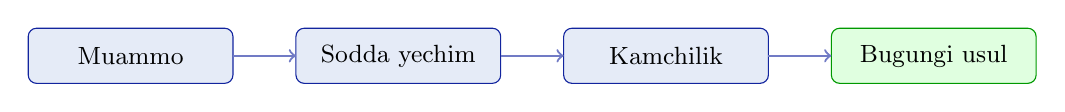
\begin{tikzpicture}
    \tikzset{
      s/.style={rectangle,draw=cnublue,rounded corners=3pt,
                fill=cnubluebg,minimum width=2.6cm,minimum height=0.7cm,align=center},
      g/.style={rectangle,draw=green!60!black,rounded corners=3pt,
                fill=green!12,minimum width=2.6cm,minimum height=0.7cm,align=center}
    }
    \node[s] at (0,0)   {\small Muammo};
    \node[s] at (3.4,0) {\small Sodda yechim};
    \node[s] at (6.8,0) {\small Kamchilik};
    \node[g] at (10.2,0){\small Bugungi usul};
    \draw[->,thick,draw=cnublue!60] (1.3,0)--(2.1,0);
    \draw[->,thick,draw=cnublue!60] (4.7,0)--(5.5,0);
    \draw[->,thick,draw=cnublue!60] (8.1,0)--(8.9,0);
  \end{tikzpicture}
  \end{center}
\end{frame}

% ================================================================
\section[Nazariya]{Nazariya: Yangi Usul}
% ================================================================

% ----------------------------------------------------------------
% [F] INTUITSIYA — avval rasm, keyin formula.
% Qoida: bu slaydda BIRORTA formula bo'lmasin.
% ----------------------------------------------------------------
\begin{frame}{Intuitsiya: G'oyani Rasmda Ko'ramiz}
  \begin{columns}
    \begin{column}{0.52\textwidth}
      \begin{center}
      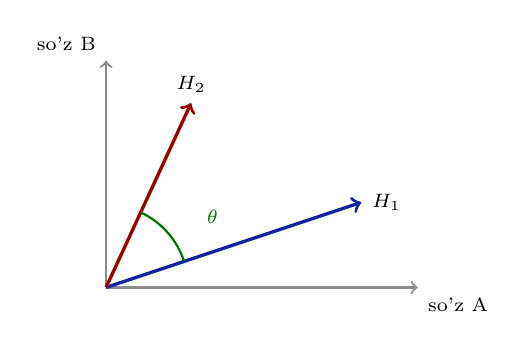
\begin{tikzpicture}[scale=0.9]
        % Misol: ikki hujjat vektorlari orasidagi burchak
        \draw[->,thick,draw=halfgray] (0,0)--(4.4,0)
              node[below right]{\scriptsize so'z A};
        \draw[->,thick,draw=halfgray] (0,0)--(0,3.2)
              node[above left]{\scriptsize so'z B};
        \draw[->,very thick,draw=cnublue]  (0,0)--(3.6,1.2)
              node[right]{\scriptsize $H_1$};
        \draw[->,very thick,draw=deepred] (0,0)--(1.2,2.6)
              node[above]{\scriptsize $H_2$};
        \draw[draw=deepgreen,thick] (1.1,0.37) arc (18:65:1.15);
        \node[color=deepgreen] at (1.5,1.0) {\scriptsize $\theta$};
      \end{tikzpicture}
      \end{center}
    \end{column}
    \begin{column}{0.44\textwidth}
      \textbf{Asosiy g'oya (so'z bilan):}
      \begin{itemize}\setlength\itemsep{4pt}
        \item Har hujjat --- fazodagi \textbf{vektor}
        \item O'xshashlik = vektorlar orasidagi \textbf{burchak}
        \item Burchak kichik $\Rightarrow$ mavzu yaqin
      \end{itemize}
      \vspace{0.2em}
      \begin{tcolorbox}[okbox]
        \small Formulaga o'tishdan oldin: g'oyani \textbf{bir gap}da
        ayta olasizmi? Ayta olsangiz --- davom etamiz.
      \end{tcolorbox}
    \end{column}
  \end{columns}
\end{frame}

% ----------------------------------------------------------------
% [G] FORMAL TA'RIF — defbox + majburiy "bunda:" kaliti
% ----------------------------------------------------------------
\begin{frame}{Formal Ta'rif}
  \begin{tcolorbox}[defbox,title=Ta'rif: kosinus o'xshashligi]
    \vspace{-0.6em}
    $$\cos(\mathbf{a},\mathbf{b})
      = \frac{\mathbf{a}\cdot\mathbf{b}}
             {\lVert\mathbf{a}\rVert\,\lVert\mathbf{b}\rVert}
      = \frac{\sum_{i=1}^{n} a_i b_i}
             {\sqrt{\sum_{i=1}^{n} a_i^2}\,\sqrt{\sum_{i=1}^{n} b_i^2}}$$
  \end{tcolorbox}
  \vspace{0.2em}
  \bunda{$\mathbf{a},\mathbf{b}\in\mathbb{R}^n$ --- hujjat vektorlari
  (masalan, TF-IDF); $n$ --- lug'at hajmi; $\mathbf{a}\cdot\mathbf{b}$
  --- skalyar ko'paytma; $\lVert\cdot\rVert$ --- Evklid normasi.}
  \vspace{0.5em}
  \begin{itemize}\setlength\itemsep{3pt}
    \item Qiymatlar oralig'i: $[-1,\,1]$; TF-IDF manfiy emas
          $\Rightarrow$ amalda $[0,\,1]$
    \item $\cos = 1$: yo'nalish bir xil; $\cos = 0$: umumiy so'z yo'q
  \end{itemize}
\end{frame}

% ----------------------------------------------------------------
% [H] KELTIRIB CHIQARISH — qadam-baqadam, har qadam izohli.
% Qoida: bitta slaydda <= 4 qadam; har qadam o'ng tomonda izoh.
% \pause faqat displaylar ORASIDA (align ichida emas).
% ----------------------------------------------------------------
\begin{frame}{Keltirib Chiqarish: Nega Aynan Shu Formula?}
  \textbf{1-qadam.} Skalyar ko'paytmaning geometrik ta'rifidan boshlaymiz:
  $$\mathbf{a}\cdot\mathbf{b}
    = \lVert\mathbf{a}\rVert\,\lVert\mathbf{b}\rVert\cos\theta
    \qquad\text{\scriptsize\color{halfgray}(chiziqli algebradan ma'lum)}$$
  \pause
  \textbf{2-qadam.} Bizga kerak bo'lgan $\cos\theta$ ni ajratib olamiz:
  $$\cos\theta
    = \frac{\mathbf{a}\cdot\mathbf{b}}
           {\lVert\mathbf{a}\rVert\,\lVert\mathbf{b}\rVert}
    \qquad\text{\scriptsize\color{halfgray}(ikkala tomonni normalarga bo'ldik)}$$
  \pause
  \textbf{3-qadam.} Nega uzunlikka bo'lish \textbf{muhim}?
  $H_1$ ni o'ziga ikki marta yopishtirsak ($\mathbf{a}' = 2\mathbf{a}$):
  $$\cos(\mathbf{a}',\mathbf{b})
    = \frac{2(\mathbf{a}\cdot\mathbf{b})}
           {2\lVert\mathbf{a}\rVert\,\lVert\mathbf{b}\rVert}
    = \cos(\mathbf{a},\mathbf{b})$$
  \begin{tcolorbox}[okbox]
    \small \textbf{Xulosa:} kosinus hujjat \textbf{uzunligiga bog'liq emas}
    --- qisqa xat va uzun maqola adolatli taqqoslanadi. Evklid
    masofasi bunday xossaga ega emas!
  \end{tcolorbox}
\end{frame}

% ----------------------------------------------------------------
% [I] QO'LDA HISOBLANGAN MISOL — kichik, to'liq, tekshiriladigan.
% Qoida: sonlar shunday tanlansinki, hisob auditoriyada og'zaki
% bajarilsin. Korpus o'zbekcha bo'lsin.
% ----------------------------------------------------------------
\begin{frame}{Qo'lda Hisoblash: To'liq Misol}
  \begin{tcolorbox}[defbox,title=Kichik korpus (BoW vektorlari)]
    \small
    $H_1$: \texttt{nlp juda qiziq} $\;\to\; \mathbf{a}=(1,1,1,0)$\quad
    $H_2$: \texttt{nlp juda foydali} $\;\to\; \mathbf{b}=(1,1,0,1)$\\[2pt]
    {\scriptsize\color{halfgray}Lug'at tartibi:
    (\texttt{nlp}, \texttt{juda}, \texttt{qiziq}, \texttt{foydali})}
  \end{tcolorbox}
  \vspace{0.2em}
  \begin{columns}
    \begin{column}{0.50\textwidth}
      \textbf{Hisoblaymiz:}
      \begin{align*}
        \mathbf{a}\cdot\mathbf{b} &= 1{\cdot}1 + 1{\cdot}1 + 1{\cdot}0 + 0{\cdot}1 = 2\\
        \lVert\mathbf{a}\rVert &= \sqrt{1+1+1+0} = \sqrt{3}\\
        \lVert\mathbf{b}\rVert &= \sqrt{1+1+0+1} = \sqrt{3}
      \end{align*}
    \end{column}
    \begin{column}{0.46\textwidth}
      \textbf{Natija:}
      $$\cos = \frac{2}{\sqrt{3}\sqrt{3}} = \frac{2}{3} \approx 0.667$$
      \begin{tcolorbox}[okbox]
        \small Ikki hujjat 4 so'zdan 2 tasida mos --- intuitsiya
        bilan ham $\approx 2/3$ chiqishi tabiiy.
      \end{tcolorbox}
    \end{column}
  \end{columns}
\end{frame}

% ----------------------------------------------------------------
% [J] "SIZNING VAZIFANGIZ" — savol -> \pause -> javob.
% Qoida: oldingi misol bilan BIR XIL ko'rinishda, sonlar boshqa.
% ----------------------------------------------------------------
\begin{frame}{Sizning Vazifangiz \textnormal{\small (2 daqiqa)}}
  \begin{tcolorbox}[warnbox,title=Savol]
    \small $H_3$: \texttt{python juda qulay}
    $\;\to\;\mathbf{c}=(0,1,0,0,1,1)$ \quad
    $H_1$: \texttt{nlp juda qiziq}
    $\;\to\;\mathbf{a}=(1,1,1,0,0,0)$\\[3pt]
    {\scriptsize\color{halfgray}Lug'at: (\texttt{nlp}, \texttt{juda},
    \texttt{qiziq}, \texttt{foydali}, \texttt{python}, \texttt{qulay})}\\[5pt]
    \textbf{\large $\cos(\mathbf{a},\mathbf{c})$ ni hisoblang.}
  \end{tcolorbox}
  \pause
  \vspace{0.3em}
  \begin{tcolorbox}[okbox,title=Javob]
    \small
    $\mathbf{a}\cdot\mathbf{c} = 1$ (faqat \texttt{juda} mos);\quad
    $\lVert\mathbf{a}\rVert = \lVert\mathbf{c}\rVert = \sqrt{3}$\\[3pt]
    $\cos = 1/3 \approx \mathbf{0.333}$ ---
    $H_3$ haqiqatan $H_2$ ga emas, $H_1$ ga ham uzoqroq:
    mavzu boshqa (\texttt{python} vs \texttt{nlp}).
  \end{tcolorbox}
\end{frame}

% ----------------------------------------------------------------
% [K] KOD <-> FORMULA KO'PRIGI
% Qoida: kod izohlarida formula qadamlarining raqamini ko'rsating.
% ----------------------------------------------------------------
\begin{frame}[fragile]{Kodda: Har Qator Formulaning Qaysi Qismi?}
  \begin{columns}
    \begin{column}{0.52\textwidth}
      \begin{lstlisting}
import numpy as np
from sklearn.metrics.pairwise \
    import cosine_similarity

a = np.array([[1, 1, 1, 0]])
b = np.array([[1, 1, 0, 1]])

# (1) skalyar ko'paytma
skalyar = (a * b).sum()      # 2
# (2) normalar
na = np.linalg.norm(a)       # 1.732
nb = np.linalg.norm(b)       # 1.732
# (3) kosinus = (1) / (2)
print(skalyar / (na * nb))   # 0.667

# bitta qatorda:
print(cosine_similarity(a, b))
      \end{lstlisting}
    \end{column}
    \begin{column}{0.44\textwidth}
      \textbf{Moslik jadvali:}
      \vspace{0.2em}
      \begin{center}\scriptsize
      \begin{tabular}{ll}
        \toprule
        \textbf{Kod} & \textbf{Formula} \\
        \midrule
        \texttt{(a*b).sum()} & $\sum_i a_i b_i$ \\
        \texttt{norm(a)} & $\lVert\mathbf{a}\rVert$ \\
        \texttt{skalyar/(na*nb)} & $\cos(\mathbf{a},\mathbf{b})$ \\
        \bottomrule
      \end{tabular}
      \end{center}
      \vspace{0.3em}
      \begin{tcolorbox}[okbox]
        \small Ertangi amaliyotda xuddi shu hisob \textbf{haqiqiy
        TF-IDF matritsada} bajariladi --- bugungi qo'lda misol
        uning birlik testi (sanity check) bo'ladi.
      \end{tcolorbox}
    \end{column}
  \end{columns}
\end{frame}

% ----------------------------------------------------------------
% [L] CHEKLOVLAR VA TIPIK XATOLAR
% Qoida: kamida bitta "tez-tez uchraydigan xato" --- kod bilan.
% ----------------------------------------------------------------
\begin{frame}[fragile]{Cheklovlar va Tipik Xatolar}
  \begin{columns}
    \begin{column}{0.50\textwidth}
      \begin{tcolorbox}[warnbox,title=Usulning cheklovlari]
        \small
        \begin{itemize}\setlength\itemsep{2pt}
          \item Sinonimlarni ko'rmaydi:
                \textit{avto} $\ne$ \textit{mashina} $\Rightarrow \cos=0$
          \item Siyrak vektorlarda ko'p nol --- xotira isrofi
          \item So'z tartibini hisobga olmaydi (BoW merosi)
        \end{itemize}
      \end{tcolorbox}
      {\scriptsize\color{halfgray}Bu kamchiliklar 4-kunda
      (embeddinglar) hal bo'ladi --- kurs shunday qurilgan.}
    \end{column}
    \begin{column}{0.46\textwidth}
      \begin{tcolorbox}[warnbox,title=Tipik xato]
        \small \texttt{cosine\_similarity} ga \textbf{1D} massiv
        berish:
      \end{tcolorbox}
      \begin{lstlisting}
a = np.array([1, 1, 1, 0])
cosine_similarity(a, b)
# XATO: Expected 2D array!

# To'g'ri: (1, n) shakl
cosine_similarity(
    a.reshape(1, -1),
    b.reshape(1, -1))
      \end{lstlisting}
    \end{column}
  \end{columns}
\end{frame}

% ----------------------------------------------------------------
% [M] O'ZBEK TILIGA XOSLIK — har ma'ruzada majburiy slayd.
% ----------------------------------------------------------------
\begin{frame}{O'zbek Tilida: Nimaga E'tibor Beramiz?}
  \begin{tcolorbox}[defbox,title=Agglutinativlik kosinusga qanday ta'sir qiladi?]
    \small \texttt{kitob}, \texttt{kitoblar}, \texttt{kitobimizdan} ---
    BoW uchun \textbf{uch xil} so'z $\Rightarrow$ aslida bir mavzuli
    hujjatlar orasida $\cos$ sun'iy past chiqadi.
  \end{tcolorbox}
  \vspace{0.3em}
  \begin{columns}
    \begin{column}{0.50\textwidth}
      \textbf{Amaliy yechimlar:}
      \begin{itemize}\setlength\itemsep{3pt}
        \item Oldindan \textbf{stemming} (o'tgan dars
              \texttt{TextPreprocessor})
        \item Qo'shimchalarni regex bilan qirqish
        \item Keyinroq: subword tokenizatsiya (BPE) --- 4-haftada
      \end{itemize}
    \end{column}
    \begin{column}{0.46\textwidth}
      \begin{center}\small
      \begin{tabular}{lcc}
        \toprule
        & \textbf{Stem'siz} & \textbf{Stem bilan} \\
        \midrule
        $\cos(H_a,H_b)$ & 0.21 & 0.58 \\
        \bottomrule
      \end{tabular}
      \end{center}
      {\scriptsize\color{halfgray}Bir xil mavzudagi ikki o'zbekcha
      yangilik matni; stemming o'xshashlikni ochib beradi.
      Ertaga amaliyotda o'zingiz tekshirasiz.}
    \end{column}
  \end{columns}
\end{frame}

% ================================================================
\section[Sintez]{Sintez va Ilmiy Manba}
% ================================================================

% ----------------------------------------------------------------
% [N] SINTEZ — kun usullarini yagona jadvalga yig'ish.
% Qoida: ustunlar = "qachon ishlatamiz" mezonlari, marketing emas.
% ----------------------------------------------------------------
\begin{frame}{Sintez: Qaysi Usulni Qachon Tanlaymiz?}
  \begin{center}\small
  \begin{tabular}{lccc}
    \toprule
    & \textbf{Evklid masofa} & \textbf{Kosinus} & \textbf{Jakkard} \\
    \midrule
    Uzunlikka sezgir & ha & \textbf{yo'q} & yo'q \\
    Chastotani hisoblaydi & ha & ha & \textbf{yo'q} \\
    Oraliq & $[0,\infty)$ & $[0,1]$ & $[0,1]$ \\
    TF-IDF bilan & o'rtacha & \textbf{standart} & mos emas \\
    Qachon & klasterlash & qidiruv, NLP & to'plamlar \\
    \bottomrule
  \end{tabular}
  \end{center}
  \vspace{0.4em}
  \begin{tcolorbox}[okbox]
    \small \textbf{Amaliy qoida:} matn + TF-IDF $\Rightarrow$ deyarli
    har doim kosinus. Istisnolarni bilish --- ekspertlik belgisi:
    juda qisqa matnlarda (tvit) Jakkard barqarorroq bo'lishi mumkin.
  \end{tcolorbox}
\end{frame}

% ----------------------------------------------------------------
% [O] ILMIY MANBA — har ma'ruzada majburiy.
% Qoida: bitta asl maqola + bitta muhokama savoli.
% ----------------------------------------------------------------
\begin{frame}{Ilmiy Manba: G'oya Qayerdan Kelgan?}
  \begin{tcolorbox}[defbox,title=Asl maqola]
    \small Salton, G., Wong, A., Yang, C.S. (1975).
    \textit{A Vector Space Model for Automatic Indexing.}
    Communications of the ACM, 18(11).
  \end{tcolorbox}
  \vspace{0.3em}
  \begin{columns}
    \begin{column}{0.50\textwidth}
      \textbf{Maqolaning hissasi:}
      \begin{itemize}\setlength\itemsep{3pt}
        \item Hujjat = vektor g'oyasini birinchi bo'lib
              tizimlashtirgan
        \item 50 yildan beri qidiruv tizimlarining asosi
        \item Bugungi RAG (4-hafta!) --- shu g'oyaning davomi
      \end{itemize}
    \end{column}
    \begin{column}{0.46\textwidth}
      \begin{tcolorbox}[warnbox,title=Muhokama savoli \textnormal{\scriptsize (keyingi darsga)}]
        \small 1975-yilgi vektor fazo modeli bilan 2013-yilgi
        Word2Vec o'rtasidagi \textbf{tub farq} nimada?
        Bir jumlada javob tayyorlang.
      \end{tcolorbox}
    \end{column}
  \end{columns}
\end{frame}

% ================================================================
\section[Xulosa]{Xulosa va Amaliyot}
% ================================================================

% ----------------------------------------------------------------
% [P] XULOSA — [C] dagi maqsadlarga belgili qaytish.
% ----------------------------------------------------------------
\begin{frame}{Xulosa: Maqsadlarga Qaytamiz}
  \begin{enumerate}\setlength\itemsep{6pt}
    \item \bajarildi \textbf{Keltirib chiqardik:} kosinus ---
          skalyar ko'paytmaning geometrik ta'rifidan
    \item \bajarildi \textbf{Qo'lda hisobladik:} $2/3$ va $1/3$
          misollari
    \item \bajarildi \textbf{Taqqosladik:} Evklid / kosinus /
          Jakkard --- tanlash mezonlari bilan
    \item \bajarildi \textbf{Kodda bog'ladik:}
          \texttt{cosine\_similarity} $\leftrightarrow$ formula
  \end{enumerate}
  \vspace{0.3em}
  \begin{tcolorbox}[defbox,title=Bitta gap bilan]
    \small Bugungi dars: \textit{hujjatlarni vektor sifatida ko'rib,
    o'xshashlikni uzunlikka bog'liq bo'lmagan burchak orqali o'lchadik.}
  \end{tcolorbox}
\end{frame}

% ----------------------------------------------------------------
% [Q] ERTANGI AMALIYOTGA KO'PRIK — ma'ruza-amaliyot bog'lovchisi.
% Qoida: (1) nima quriladi, (2) bugungi qaysi formula ishlatiladi,
% (3) nima tayyorlab kelish kerak.
% ----------------------------------------------------------------
\begin{frame}{Ertaga Amaliyotda \textnormal{\small (09:30, I.R.Atadjanov)}}
  \begin{center}
  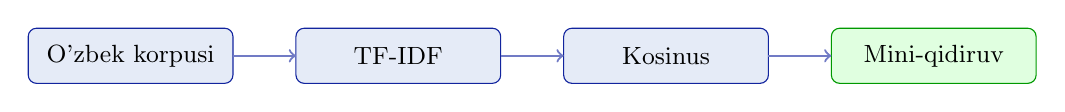
\begin{tikzpicture}
    \tikzset{
      s/.style={rectangle,draw=cnublue,rounded corners=3pt,
                fill=cnubluebg,minimum width=2.6cm,minimum height=0.7cm,align=center},
      g/.style={rectangle,draw=green!60!black,rounded corners=3pt,
                fill=green!12,minimum width=2.6cm,minimum height=0.7cm,align=center}
    }
    \node[s] at (0,0)   {\small O'zbek korpusi};
    \node[s] at (3.4,0) {\small TF-IDF};
    \node[s] at (6.8,0) {\small Kosinus};
    \node[g] at (10.2,0){\small Mini-qidiruv};
    \draw[->,thick,draw=cnublue!60] (1.3,0)--(2.1,0);
    \draw[->,thick,draw=cnublue!60] (4.7,0)--(5.5,0);
    \draw[->,thick,draw=cnublue!60] (8.1,0)--(8.9,0);
  \end{tikzpicture}
  \end{center}
  \vspace{0.2em}
  \begin{columns}
    \begin{column}{0.50\textwidth}
      \textbf{Quriladi:} loyihangizning navbatdagi moduli ---
      so'rov bo'yicha eng yaqin hujjatni topuvchi qidiruv.
      \vspace{0.2em}
      \begin{itemize}\setlength\itemsep{2pt}
        \item Bugungi [G] formula --- kodning yadrosi
        \item [I] misol --- birlik test sifatida
      \end{itemize}
    \end{column}
    \begin{column}{0.46\textwidth}
      \begin{tcolorbox}[warnbox,title=Tayyorlab keling]
        \small
        \begin{itemize}\setlength\itemsep{1pt}
          \item Kaggle hisobingiz ishlashini tekshiring
          \item O'tgan amaliyot notebook'i ochilsin
          \item Muhokama savoliga [O] javob
        \end{itemize}
      \end{tcolorbox}
    \end{column}
  \end{columns}
\end{frame}

% ----------------------------------------------------------------
% [R] ADABIYOTLAR
% ----------------------------------------------------------------
\begin{frame}{Adabiyotlar va Qo'shimcha O'qish}
  \small
  \begin{enumerate}\setlength\itemsep{4pt}
    \item Jurafsky, D., Martin, J. \textit{Speech and Language
          Processing} (3-nashr loyihasi) --- 6-bob.
    \item Salton, G. va b. (1975). \textit{A Vector Space Model
          for Automatic Indexing}. CACM 18(11).
    \item Manning, C. va b. \textit{Introduction to Information
          Retrieval} --- 6.3-bo'lim (onlayn bepul).
  \end{enumerate}
  \vspace{0.5em}
  {\scriptsize\color{halfgray}Kurs materiallari: GitHub repozitoriy
  manzili shu yerda. Savollar: elektron pochta.}
\end{frame}

% ----------------------------------------------------------------
% [S] ZAXIRA SLAYDLAR — \appendix dan keyin; raqamlanish asosiy
% hisobga kirmaydi. Bu yerga: matematik eslatmalar, qo'shimcha
% isbotlar, chuqurroq savollarga javoblar.
% ----------------------------------------------------------------
\appendix

\begin{frame}{Zaxira: Logarifm Xossalari Eslatmasi}
  \begin{tcolorbox}[defbox,title=Kerakli xossalar]
    \small
    $\ln(ab) = \ln a + \ln b$;\qquad
    $\ln(a/b) = \ln a - \ln b$;\qquad
    $\ln 1 = 0$;\qquad
    $a > b > 0 \Rightarrow \ln a > \ln b$
  \end{tcolorbox}
  \vspace{0.3em}
  \small IDF formulasida $\ln(N/\mathrm{df})$ ishlatilishining sababi:
  hujjatlar soni o'sganda og'irlik \textbf{sekin} o'sishi kerak ---
  chiziqli emas, logarifmik.
\end{frame}

\begin{frame}{Zaxira: Nega $\cos$ TF-IDF bilan ``standart''?}
  \small TF-IDF vektorlari manfiy emas va odatda $L_2$-normallashtiriladi.
  Normallashtirilgan vektorlar uchun:
  $$\lVert\mathbf{a}-\mathbf{b}\rVert^2
    = \lVert\mathbf{a}\rVert^2 + \lVert\mathbf{b}\rVert^2
      - 2\,\mathbf{a}\cdot\mathbf{b}
    = 2 - 2\cos(\mathbf{a},\mathbf{b})$$
  \bunda{$\lVert\mathbf{a}\rVert=\lVert\mathbf{b}\rVert=1$ deb olindi.}
  \vspace{0.3em}

  Demak, normallashtirilgan fazoda Evklid masofasi va kosinus
  \textbf{ekvivalent tartib} beradi --- shuning uchun
  \texttt{scikit-learn} ko'pincha ikkalasini almashtirib ishlatadi.
\end{frame}

\end{document}
